%% This file was auto-generated by IPython.
%% Conversion from the original notebook file:
%% level2.ipynb
%%
\documentclass[11pt,english,fleqn]{article}

%% This is the automatic preamble used by IPython.  Note that it does *not*
%% include a documentclass declaration, that is added at runtime to the overall
%% document.

\usepackage{amsmath}
\usepackage{amssymb}
\usepackage{graphicx}
\usepackage{ucs}
\usepackage[utf8x]{inputenc}

% needed for markdown enumerations to work
\usepackage{enumerate}

% Slightly bigger margins than the latex defaults
\usepackage{geometry}
\geometry{verbose,tmargin=3cm,bmargin=3cm,lmargin=2.5cm,rmargin=2.5cm}

% Define a few colors for use in code, links and cell shading
\usepackage{color}
\definecolor{orange}{cmyk}{0,0.4,0.8,0.2}
\definecolor{darkorange}{rgb}{.71,0.21,0.01}
\definecolor{darkgreen}{rgb}{.12,.54,.11}
\definecolor{myteal}{rgb}{.26, .44, .56}
\definecolor{gray}{gray}{0.45}
\definecolor{lightgray}{gray}{.95}
\definecolor{mediumgray}{gray}{.8}
\definecolor{inputbackground}{rgb}{.95, .95, .85}
\definecolor{outputbackground}{rgb}{.95, .95, .95}
\definecolor{traceback}{rgb}{1, .95, .95}

% Framed environments for code cells (inputs, outputs, errors, ...).  The
% various uses of \unskip (or not) at the end were fine-tuned by hand, so don't
% randomly change them unless you're sure of the effect it will have.
\usepackage{framed}

% remove extraneous vertical space in boxes
\setlength\fboxsep{0pt}

% codecell is the whole input+output set of blocks that a Code cell can
% generate.

% TODO: unfortunately, it seems that using a framed codecell environment breaks
% the ability of the frames inside of it to be broken across pages.  This
% causes at least the problem of having lots of empty space at the bottom of
% pages as new frames are moved to the next page, and if a single frame is too
% long to fit on a page, will completely stop latex from compiling the
% document.  So unless we figure out a solution to this, we'll have to instead
% leave the codecell env. as empty.  I'm keeping the original codecell
% definition here (a thin vertical bar) for reference, in case we find a
% solution to the page break issue.

%% \newenvironment{codecell}{%
%%     \def\FrameCommand{\color{mediumgray} \vrule width 1pt \hspace{5pt}}%
%%    \MakeFramed{\vspace{-0.5em}}}
%%  {\unskip\endMakeFramed}

% For now, make this a no-op...
\newenvironment{codecell}{}

 \newenvironment{codeinput}{%
   \def\FrameCommand{\colorbox{inputbackground}}%
   \MakeFramed{\advance\hsize-\width \FrameRestore}}
 {\unskip\endMakeFramed}

\newenvironment{codeoutput}{%
   \def\FrameCommand{\colorbox{outputbackground}}%
   \vspace{-1.4em}
   \MakeFramed{\advance\hsize-\width \FrameRestore}}
 {\unskip\medskip\endMakeFramed}

\newenvironment{traceback}{%
   \def\FrameCommand{\colorbox{traceback}}%
   \MakeFramed{\advance\hsize-\width \FrameRestore}}
 {\endMakeFramed}

% Use and configure listings package for nicely formatted code
\usepackage{listingsutf8}
\lstset{
  language=python,
  inputencoding=utf8x,
  extendedchars=\true,
  aboveskip=\smallskipamount,
  belowskip=\smallskipamount,
  xleftmargin=2mm,
  breaklines=true,
  basicstyle=\small \ttfamily,
  showstringspaces=false,
  keywordstyle=\color{blue}\bfseries,
  commentstyle=\color{myteal},
  stringstyle=\color{darkgreen},
  identifierstyle=\color{darkorange},
  columns=fullflexible,  % tighter character kerning, like verb
}

% The hyperref package gives us a pdf with properly built
% internal navigation ('pdf bookmarks' for the table of contents,
% internal cross-reference links, web links for URLs, etc.)
\usepackage{hyperref}
\hypersetup{
  breaklinks=true,  % so long urls are correctly broken across lines
  colorlinks=true,
  urlcolor=blue,
  linkcolor=darkorange,
  citecolor=darkgreen,
  }

% hardcode size of all verbatim environments to be a bit smaller
\makeatletter 
\g@addto@macro\@verbatim\small\topsep=0.5em\partopsep=0pt
\makeatother 

% Prevent overflowing lines due to urls and other hard-to-break entities.
\sloppy

\setlength{\mathindent}{0pt}
\setlength{\parindent}{0pt}
\setlength{\parskip}{8pt}
\begin{document}

Kesit Seviyeleri, Kenar Bazli Imaj Gruplamak

Bir dijital imaji renklere, objelere gore belli parcalara bolmek
(segmentation) icin, matematiksel bir formul kullanmak iyi cozumlerden
biridir. Bunu yapmanin bazi yollari var. Basitlestirerek bir ornek
verelim: diyelim ki gruplama icin elimizdeki formul bir yuvarlak formulu
$x^2+y^2 - c = 0$, ki $c$ bir sabit. Bu formulu x ve y kordinatlari
uzerinde bastigimiz zaman radius'u $\sqrt{c}$ olan bir cember elde
ederiz. Gruplama icin bu cemberi buyutup kucultebildigimizi farzedelim,
cember imaj uzerindeki istedigimiz bolume en iyi uydugu anda gruplamayi
basarili olarak kabul ediyoruz.

Fakat problem surada: eger imajda birden fazla grup var ise, o zaman
birden fazla cember gerekecektir, bu sefer algoritmik olarak ustteki
formulu ikinci, ucuncu kere yaratmamiz, ve o formullerin o gruplara
uyumunu ayri ayri takip etmemiz gerekirdi. Ya da diyelim ki ozyineli
(iterative) bir uydurma islemi takip ediyoruz, bu islem sirasinda belki
iki cemberin birlesmesi gerekse, o zaman iki formulu silip, yerine
yenisini olusturmakla ugrasmak gerekli olacakti. Bunlar hem
matematiksel, hem kodlama acisindan kulfet olusturacaktir.

Kesit Seviyeleri kavramini kullanarak bu isi daha basitlestirebiliriz.
Diyelim ki bolme gorevini yapan $\phi$ adli fonksiyonumuzu 2 boyutlu
olmak yerine 3 boyutlu eksende tanimladik, ve, 2 boyutta bolme yapma
gorevini onun bir kesitine verdik. Kesit derken, alttaki uc boyutlu
fonksiyonu yatay olarak bir noktadan ``kestigimizi'' farz ediyoruz, ve o
kesit uzerinde dusen $\phi$ degerlerine bakiyoruz.

Bakic acisimizi, tanimlamamizi degistirerek, bazi avantajlar elde etmeyi
umuyoruz aslinda. Altta iki tane $\phi$ fonksiyonu ve onlarin altinda
kesitlerini gorebiliriz.

Kesit Seviyeleri teknigini kullanarak elde ettigimiz avantaj nedir?
Artik sadece \textbf{tek} bir $\phi$ fonksiyonu kullanarak 2 boyutlu
imajimiz uzerinde birbirinden ayri gruplamalar yaratabiliyoruz. Bu
gruplar birbiri ile birlesebilir, ayrilabilir, bu artik bizi
ilgilendirmiyor. Biz sadece 3. boyuttaki $\phi$ fonksiyonunu
degistirmekle ugrasacagiz, imaj uzerindeki gruplamalar ise o fonksiyonun
2. boyuta yansimasi (projection) uzerinden kendiliginden
gerceklesecekler.

Matematiksel olarak $\phi$ fonksiyonunu nasil temsil ederiz? $\phi$
fonksiyonu $x$, $y$, boyutlarini alip bize bir ucuncu $z$ boyutu
dondurmeli, ayrica bu fonksiyonu imaji parcalarina ayirma islemini
gerceklestirmek icin kademeli olarak degistirmeyi planladigimiza gore, o
zaman bir $t$ degiskeni de gerekiyor. Yani $\phi(x,y,t)$ fonksiyonu.
Gruplama icin kullanilacak kesiti ise sifir kesiti olarak alalim, yani
$\phi(x,y,t) = 0$. Dogal olarak
\[ \frac{d}{dt}(\phi(x,y,t) = 0) = 0 \]
Simdi $x$, ve $y$ degiskenlerinin zaman gore degisimini formule bir
sekilde dahil etmek lazim. Bunun icin sifir kesit seviyesi uzerinde bir
parcacik hayal edilir, ve bu parcacigin gittigi yol $x(t)$, ve $y(t)$
olarak tanimlanir. O zaman
\[ \frac{d}{dt}(\phi(x(t),y(t),t) = 0) = 0 \]
Tam diferansiyel formulunden hareketle:
\[ 
d(\phi(x(t),y(t),t) = 
\frac{\partial \phi}{\partial x}dx + 
\frac{\partial \phi}{\partial y}dy + 
\frac{\partial \phi}{\partial t}dt  = 0
 \]\[ 
\frac{d(\phi(x(t),y(t),t))}{dt} = 
\frac{\partial \phi}{\partial x}\frac{dx}{dt} + 
\frac{\partial \phi}{\partial y}\frac{dy}{dt} + 
\frac{\partial \phi}{\partial t} = 0
 \]
\begin{equation} \frac{d(\phi(x(t),y(t),t))}{dt} = 
\frac{\partial \phi}{\partial x}\frac{dx}{dt} + 
\frac{\partial \phi}{\partial y}\frac{dy}{dt} + 
\phi_t = 0\label{eq1} 
\end{equation}

Temsilen daha kisa bir isaret kullanmak gerekirse, $\bigtriangledown$
ile $\phi$'nin gradyanini (gradient) alarak, elde edilecek vektorun
nokta carpimini kullanabiliriz. O zaman formul\ensuremath{\sim}\ref{eq1}
daha kisa olarak:
\[ \phi_t + \bigtriangledown \phi \cdot \vec{V} = 0 \]
olarak temsil edilebilir, ki
\[ \bigtriangledown \phi = \bigg(
\frac{\partial \phi}{\partial x},
\frac{\partial \phi}{\partial y} \bigg)
 \]\[ \vec{V} = \bigg(
\frac{dx}{dt} ,
\frac{dy}{dt} \bigg)
 \]
Iki vektorun nokta carpimi bilindigi gibi sirayla her iki vektorun
sirasiyla uyan elemanlarinin birbirleri ile carpilmasi ve o carpimlarin
toplanmasidir.

$\vec{V}$ vektoru neyi temsil eder? Formule gore bu vektor $\phi$`nin
uzerindeki degisimi etkiliyor, ve bu degisimler $t$'nin degisimine gore
tanimlandigina gore bu degerler ``hiz'' olarak tanimlanabilir. Imaj
baglaminda dusunursek mesela $\phi$ renklerin ayni oldugu yerlerde
yuksek hizda, renklerin degistigi yerler dusuk hizda degisebilir
seklinde bir kurgu yapilabilir, iste bu bolgelerde degisiminin hizini
$\vec{V}$ ile gosterebiliriz.

$\vec{V}$ yerine kesit seviyelerine dik olan (normal) vektorler ile
calismak isteseydik, $\vec{V}$'yi dik ve teget bilesenlerine ayirarak
tekrar temsil edebilirdik: $\vec{V} = V_N\vec{N} + V_T\vec{T}$. Bu
formulde $\vec{T}$ teget, $\vec{N}$ dik vektorler, $N$ ve $T$ skalar.
Yerine koyalim:
\[ \phi_t + \bigtriangledown \phi \cdot (V_N\vec{N} + V_T\vec{T}) = 0 \]
$\phi$'ye gore dik vektorun diger bir formulu
$\vec{N} = \frac{\bigtriangledown\phi}{|\bigtriangledown\phi|}$ olduguna
gore
\[ \phi_t + (\bigtriangledown \phi \cdot
V_N\frac{\bigtriangledown\phi}{|\bigtriangledown\phi|} + \bigtriangledown
\phi \cdot V_T\vec{T}) = 0 \]
Devam edelim: $\bigtriangledown \phi$ yuzeye dik olduguna gore, bu dik
vektorun teget olan $\vec{T}$ ile noktasal carpimi sifir degerini
verecektir, o carpim formulden atilabilir. Kalanlar:
\[ \phi_t + (\bigtriangledown \phi \cdot 
V_N\frac{\bigtriangledown\phi}{|\bigtriangledown\phi|}) = 0 \]
Daha da kisaltabiliriz:
$\bigtriangledown \phi \cdot \bigtriangledown \phi = |\bigtriangledown \phi|^2$
oldugunu biliyoruz, gradyanin kendisi ile noktasal carpimi, o gradyan
vektorunun uzunlugunun karesidir. Daha genel olarak, bir vektorun
uzunlugu, o vektorun kendisi ile noktasal carpiminin karekokudur. Ayni
sey. O zaman en son formulde bu carpimi gerceklestirip, uzunluk olarak
yazalim:
\[ \phi_t + V_N\frac{|\bigtriangledown\phi|^2}{|\bigtriangledown\phi|} = 0  \]\[ \phi_t + V_N |\bigtriangledown\phi| = 0  \]
Simdi bu formul hakkinda biraz anlayis gelistirelim. Eger elimizdeki bir
$\phi$ seviye kesitinin seklen oldugu gibi kalmasini ama sadece
kuculmesini isteseydik, $\phi$'nin normalinin tersi yonunde bir buyume
tanimlamamiz gerekirdi. Normal vektor disa dogru isaret ettigine gore
ustteki formulde mesela $V_N = -1$ tanimlayabilirdik. O zaman
\[ \phi_t + -1 |\bigtriangledown\phi| = 0 \]\[ \phi_t = |\bigtriangledown\phi|   \]
Hesapsal olarak bunu nasil gerceklestiririz? 80 x 80 boyutunda bir
matris icinde $\phi$ fonksiyonu ayriksal olarak tutalim. Yani 80 tane x,
80 tane ayri y degeri var, her x ve y degerlerin kombinasyonlarina
tekabul eden $\phi$ degerleri bu matris icinde. Gradyanin ne oldugunu
hatirlayalim. Gradyan
\[ 
\bigtriangledown \phi = \bigg(
\frac{\partial \phi}{\partial x},
\frac{\partial \phi}{\partial y} \bigg)
\]
olarak tanimlidir, ve her $(x_i,y_i)$ noktasindaki $\phi(x_i,y_i)$
degerine gore degisik bir vektor sonucunu getirecektir. Bilgisayar
dunyasinda parcali turevler hesapsal ``farkliliklara'' donusurler, phi
matrisindeki farkliliklari Python ile

gradPhiY, gradPhiX = np.gradient(phi)

olarak hesaplayabiliriz. Ustte elimize gecen gradyan dizinlerindeki
degerler ile $|\bigtriangledown\phi|$ buyuklugunu hesaplayabiliriz, ve
bu sonucu $\phi$ uzerindeki degisim orani $\phi_t$ olarak kabul ederiz.
O zaman $\phi_t$ ile zaman $t$ degimi \verb!dt! carptigimiz zaman ele
gececek olan $\phi$'nin degisimidir. Dongunun her basamaginda eski
\verb!phi! degerlerine bu farklari ekledigimiz zaman $\phi$ fonksiyonu
istedigimiz gibi evrilecektir.

Alttaki kodda bizim baslangic $\phi$'miz kenarlardan w uzakliginda ici
bos bir kutu olacak.

Ortalama Egim (Mean Curvature) Kullanmak

Eger sabit hiz yerine sifir kesit seviyesinin herhangi bir noktada ne
kadar ``egri'' olduguna gore ilerlemesini isletseydik ne olurdu? Diyelim
ki cok egri bolgelerde cok hizli, az egik (duz, duze yakin) bolgelerde
ilerleme az hiz istiyoruz. O zaman hangi sekille baslarsa baslasindalar
$\phi$ kesiti sonucta bir cember sekline dogru evrilecektir. Ortalama
egim (mean curvature) hesabi icin su denklem kullanilir:
\[ \kappa = -div \bigg( \frac{\bigtriangledown \phi}
{|\bigtriangledown \phi| } \bigg) \]
\begin{codecell}
\begin{codeinput}
\begin{lstlisting}
import time
from IPython.display import clear_output
f, ax = plt.subplots()

# initial function phi - level set is a square 4 pixels
# away from borders on each side, in 3D it looks like an empty
# box
c0=2; w=2
nrow, ncol= (30,30)
phi=c0*np.ones((nrow,ncol))
phi[w+1:-w-1, w+1:-w-1]=-c0

dt=1.

phiOld=np.zeros((nrow,ncol))

iter=0

while iter < 50:
    # gradient of phi
    gradPhiY, gradPhiX = np.gradient(phi)
    # magnitude of gradient of phi
    absGradPhi=np.sqrt(gradPhiX**2+gradPhiY**2)                               
    
    # normalized gradient of phi - eliminating singularities
    normGradPhiX=gradPhiX/(absGradPhi+(absGradPhi==0))
    normGradPhiY=gradPhiY/(absGradPhi+(absGradPhi==0))
    
    divYnormGradPhiX, divXnormGradPhiX=np.gradient(normGradPhiX)
    divYnormGradPhiY, divXnormGradPhiY=np.gradient(normGradPhiY)
                           
    # curvature is the divergence of normalized gradient of phi
    K = divXnormGradPhiX + divYnormGradPhiY
    dPhiBydT = K * absGradPhi # makes everything circle
    
    # level set evolution equation    
    phi = phi + ( dt * dPhiBydT )
    iter=iter+1
    time.sleep(0.6)
    CS = ax.contour(phi,0, colors='r') 
    clear_output()
    display(f)
    ax.cla()
    iter += 1

plt.close()

\end{lstlisting}
\end{codeinput}
\begin{codeoutput}
\begin{center}
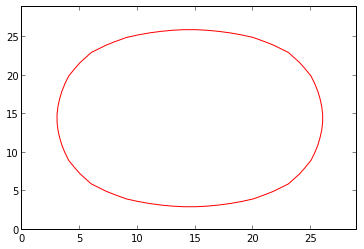
\includegraphics[width=0.7\textwidth]{level2_files/level2_fig_00.png}
\par
\end{center}
\end{codeoutput}
\end{codecell}
Imaj Gruplamak

Imaji bolumlere ayirmak icin (segmentation) birkac faktorun bilesimi
kullaniliyor. Koseleri kullanan aktif kontr (edge based active contour)
yonteminde ortalama egim ve imajin piksel degerlerinin farkliliklari
(image gradient) ayni anda kullanilir. Yani kesit seviyesini
ilerletirken hizi hem egime oranliyoruz, hem de imaj piksel renk
degerleri arasindaki farka ters oranda hizlandiriyor, ya da
yavaslatiyoruz. Boylece kesit seviyemiz renk farkliligi cok olmayan yani
buyuk bir ihtimalle tek bir objeye ait bir bolgede hizla ilerliyor,
buyuk renk farkinin oldugu buyuk bir ihtimalle bir kenar noktasina
gelince ise yavasliyor. O sirada kesit seviyesinin geri kalan taraflari
tabii ki baska hizlarda hareket ediyor olabilirler, zaten isin puf
noktasi burada, sonunda resim bolgelere ayrilmis oluyor.

Bitirirken onemli gozlemi vurgulayalim. Problemi matematiksel olarak
temsil ederken, hedefe dogru turetirken surekli (continous) alemde,
surekli, kesintisiz fonksiyonlarla is yapiyoruz. Hesaplama ani gelince
surekli fonksiyonlari ayriksal (discrete) hale ceviriyoruz, iste
uygulamali matematigin hesapsal kismi burada devreye giriyor. Fakat
diferansiyel denklemler, fonksiyonlar, turevler gibi surekli matematigin
kavramlari cok onemli, bunlar olmasa problemi soyut bir sekilde temsil
edemez, ve basitlestiremezdik. Temel matematigin kavramlarini
kullanirken yuzyillarin matematiksel bilgisi devreye girebiliyor,
matematigin en yogun sekilde kullanildigi fizikten bol bol teknik
alinabilir. Yani soylemek istedigimiz problemi cozmek icin hemen
kodlamaya baslamiyoruz, dusunsel eylemin onemli bir kismi matematiksel
formullerle (belki kalem kagitla) yapiliyor.

\begin{codecell}
\begin{codeinput}
\begin{lstlisting}
import scipy.signal as signal
import scipy.ndimage as image
import time
from scipy import ndimage
from IPython.display import clear_output
f, ax = plt.subplots()

def bwdist(a):
    """ 
    this is an intermediary function, 'a' has only True, False vals, 
    so we convert them into 0, 1 values -- in reverse. True is 0, 
    False is 1, distance_transform_edt wants it that way.
    """
    b = np.ones(a.shape)
    b[a==True] = 0.
    return ndimage.distance_transform_edt(b)

def gauss_kern():
    """ Returns a normalized 2D gauss kernel array for convolutions """
    h1 = 15
    h2 = 15
    x, y = np.mgrid[0:h2, 0:h1]
    x = x-h2/2
    y = y-h1/2
    sigma = 1.5
    g = np.exp( -( x**2 + y**2 ) / (2*sigma**2) );
    return g / g.sum()

Img = plt.imread("twoObj.bmp")
Img = Img[::-1] 
g = gauss_kern()
Img_smooth = signal.convolve(Img,g,mode='same')
Iy,Ix=np.gradient(Img_smooth)
absGradI=np.sqrt(Ix**2+Iy**2);
rows, cols = Img.shape

# initial function phi - level set is a square 4 pixels
# away from borders on each side, in 3D it looks like an empty
# box
c0=4
w=4
nrow, ncol=Img.shape
phi=c0*np.ones((nrow,ncol))
phi[w+1:-w-1, w+1:-w-1]=-c0

# edge-stopping function
g = 1 / (1+absGradI**2)

# gradient of edge-stopping function
gy,gx = np.gradient(g)

# gradient descent step size
#dt=.4
dt=1.

# number of iterations after which we reinitialize the surface
num_reinit=10

phiOld=np.zeros((rows,cols))

# number of iterations after which we reinitialize the surface
iter=0

while True:
    # gradient of phi
    gradPhiY, gradPhiX = np.gradient(phi)    
    # magnitude of gradient of phi
    absGradPhi=np.sqrt(gradPhiX**2+gradPhiY**2)
    # normalized gradient of phi - eliminating singularities
    normGradPhiX=gradPhiX/(absGradPhi+(absGradPhi==0))
    normGradPhiY=gradPhiY/(absGradPhi+(absGradPhi==0))
    
    divYnormGradPhiX, divXnormGradPhiX=np.gradient(normGradPhiX)
    divYnormGradPhiY, divXnormGradPhiY=np.gradient(normGradPhiY)
                           
    # curvature is the divergence of normalized gradient of phi
    K = divXnormGradPhiX + divYnormGradPhiY
    tmp1 = g * K * absGradPhi
    tmp2 = g * absGradPhi
    tmp3 = gx * gradPhiX + gy*gradPhiY
    dPhiBydT =tmp1 + tmp2 + tmp3    
    
    phiOld=phi
    # level set evolution equation    
    phi = phi + ( dt * dPhiBydT )
    iter=iter+1
    if np.mod(iter,num_reinit)==0:
        # reinitialize the embedding function 
        # after num_reinit iterations
        phi=np.sign(phi)
        phi = (phi > 0) * (bwdist(phi < 0)) - \
            (phi < 0) * (bwdist(phi > 0))
        
    if np.mod(iter,5)==0:
        time.sleep(0.6)
        ax.imshow(Img, cmap='gray')
        CS = ax.contour(phi,0, colors='r') 
        clear_output()
        display(f)
        ax.cla()

    if iter > 70:
        break

plt.close()

\end{lstlisting}
\end{codeinput}
\begin{codeoutput}
\begin{center}
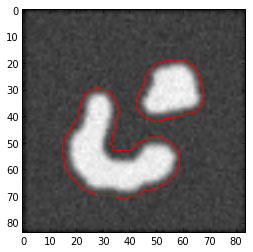
\includegraphics[width=0.7\textwidth]{level2_files/level2_fig_01.png}
\par
\end{center}
\end{codeoutput}
\end{codecell}

\end{document}
